\documentclass[xcolor=table]{beamer}
\usetheme{Madrid}
\usepackage{amssymb}
\usepackage{epsfig}
\usepackage{psfrag}
\usepackage{wrapfig}
\usepackage{graphicx}
\usepackage{color}
\usepackage{amsmath}
\usepackage{multimedia}
%\usepackage{style}
\usepackage{verbatim}
\usepackage{listings}
\usepackage{multicol}
\usepackage[table]{xcolor}

\DeclareSymbolFont{nosets}{U}{msb}{m}{7}
\DeclareMathSymbol{\natural}{\mathalpha}{nosets}{'116} %can be done with \Bbb see page 218
\DeclareMathSymbol{\real}{\mathalpha}{nosets}{'122}
\DeclareMathSymbol{\complex}{\mathalpha}{nosets}{'103}
\DeclareMathSymbol{\integer}{\mathalpha}{nosets}{'132}
\newcommand{\cross}{\wedge}
\newcommand{\vecdiv}{\nabla \cdot}
\newcommand{\grad}{\nabla}
\newcommand{\curl}{\nabla \cross}
\newcommand{\ifff}{\Leftrightarrow} % \iff is already used
\newcommand{\sgn}{\text{sgn}}
\newcommand{\vect}[1]{\mathbf{#1}}
\newcommand{\sectref}[1]{\S\ref{#1}}
\providecommand{\norm}[1]{\lVert#1\rVert}
\numberwithin{equation}{section}
\usefonttheme{professionalfonts}
%\usefonttheme[stillsansseriflarge,stillsansserifsmall]{serif}


\lstset{language=C++}
\lstset{otherkeywords={<<<,>>>}}
\lstset{morekeywords={dim3,__host__,__kernel__,__global__,__device__}}
\lstset{breaklines,breakatwhitespace,breakautoindent=false,showstringspaces=false}
\lstset{keywordstyle=\color{purple}}
\lstset{identifierstyle=\color{blue}}
\lstset{basicstyle=\fontfamily{pcr}\fontsize{9pt}{9pt}\selectfont}
%\lstset{numbers=left, numberstyle=\tiny, stepnumber=1, numbersep=5pt}
\lstset{linewidth=4.9in,xleftmargin=10pt}

\definecolor{lightblue}{rgb}{0.0,0.45,0.81}
\definecolor{lighterblue}{rgb}{0.415,0.678,0.894}
\definecolor{darkblue}{rgb}{0,0.243,0.447}
\setbeamercolor{frametitle}{bg=lightblue,fg=white}
\setbeamerfont{normal text}{family=helvet}
\setbeamerfont{local structure}{family=helvet}

\setbeamercolor*{author in head/foot}{bg=darkblue}
\setbeamercolor*{logo in head/foot}{bg=darkblue,fg=white}
\setbeamercolor*{title in head/foot}{bg=darkblue,fg=white}
\setbeamercolor*{date in head/foot}{bg=darkblue,fg=white}
\setbeamercolor{title}{bg=darkblue}
\setbeamercolor{under headline}{bg=lighterblue}
\setbeamercolor{footline}{bg=darkblue}

\setbeamerfont*{title in head/foot}{size=\small}
\setbeamerfont*{date in head/foot}{size=\small}


\setbeamertemplate{frametitle}
{
  \leavevmode%
  \begin{beamercolorbox}[wd=\paperwidth,ht=1cm]{frametitle}
   \hspace{1em}\insertframetitle\vspace{0.35cm}
   \end{beamercolorbox}%
   \vskip-0.4cm%
  \begin{beamercolorbox}[wd=\paperwidth,ht=1ex]{under headline}%
    \end{beamercolorbox}%
	
}

%\setbeamerfont{frametitle}{series=\bfseries}
\setbeamertemplate{footline}
{
  \leavevmode%
  \hbox{%
  \begin{beamercolorbox}[wd=.3\paperwidth,ht=0.8cm,center,dp=1ex]{logo in
    head/foot}%
  \usebeamerfont{logo in head/foot}
\includegraphics[width=.25\paperwidth]{./UClogo_bg.png}%
\end{beamercolorbox}%
  \begin{beamercolorbox}[wd=.28\paperwidth,center,dp=1ex,ht=0.8cm]{title in head/foot}%
    \usebeamerfont{title in head/foot}Finite Volume Methods\vspace{0.3cm}
  \end{beamercolorbox}%
  \begin{beamercolorbox}[wd=.35\paperwidth,dp=1ex,center,ht=0.8cm]{date in head/foot}%
    \usebeamerfont{date in head/foot}Laboratory for Scientific
    Computing\vspace{0.05cm}
\end{beamercolorbox}%
\begin{beamercolorbox}[wd=0.07\paperwidth,ht=0.8cm,dp=1ex,right,topskip=1em]{date
    in head/foot}%
    \insertframenumber{} / \inserttotalframenumber\hspace*{2ex}\vspace{0.3cm}
  \end{beamercolorbox}}%
  \vskip0pt%
}



\title[Beamer Intro]{Introduction to the \LaTeX{} Beamer Package}
\author{Philip Blakely}
\institute[LSC]{Laboratory for Scientific Computing, University of Cambridge}
\date{\today}
\begin{document}
\begin{frame}
  \titlepage
  \begin{tabbing}
    Thanks to:  \= Dr Nikos Nikiforakis (Supervisor)\\
    \>Coffee
  \end{tabbing}
\end{frame}

\begin{frame}{Outline}
\begin{itemize}
\item Why we need Beamer
\item How to use Beamer
\item What Beamer can produce
\item Conclusions
\end{itemize}
\end{frame}

\begin{frame}{Background}
\begin{itemize}[<+->]
\item Microsoft Powerpoint is capable of producing pretty
  presentations.
\item However it has a few drawbacks:
\begin{itemize}
\item Proprietary / costs money
\item Binary format
\item Hard to produce good equations (although more recent versions
  have improved on this)
\item Windows-based
\end{itemize}
\item We would like to be able to copy-paste equations and text from
  our \LaTeX{} reports into presentations.
\end{itemize}
\end{frame}

\begin{frame}{Beamer}
\begin{itemize}
\item Beamer is a set of \LaTeX{} packages that produce good PDF
  presentations.
\item Freely available with standard \LaTeX{} distributions
\item They are easily customisable
\item Full information easily available at\\
 \url{http://www.ctan.org/tex-archive/macros/latex/contrib/beamer/doc/beameruserguide.pdf}
\end{itemize}
\end{frame}

\begin{frame}{Equations / Algorithm}
I have proved that
\begin{equation*}
\frac{\pi^2}{6} = \sum_{n=1}^\infty \frac{1}{n^2}
\end{equation*}
\end{frame}

\begin{frame}{Results}
Using the ENO scheme to solve Burger's equation:
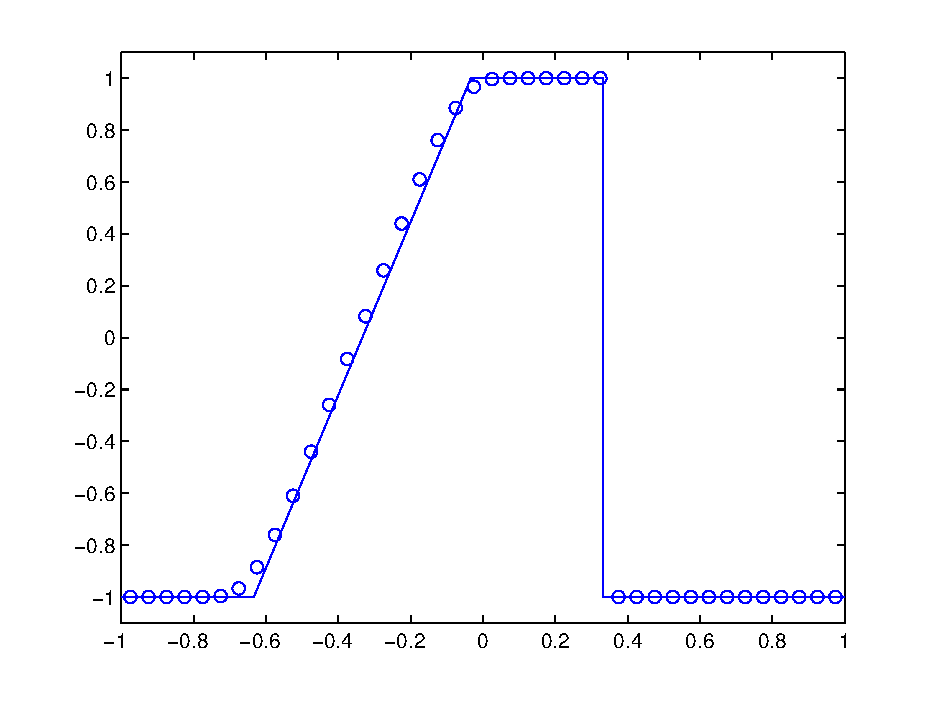
\includegraphics[width=3in]{ENOTest5.pdf}
\end{frame}

\begin{frame}{Conclusions and Further Work}
\begin{itemize}
\item Beamer allows basic and complex presentations
\item They look professional and allow the inclusion of equations
\item Movies are more of a challenge, and I am looking into this.
\end{itemize}
\end{frame}


\end{document}
